\documentclass{article}
\usepackage[utf8]{inputenc}
\usepackage[T1]{fontenc}
\usepackage[russian]{babel}
\usepackage{tikz}
\usepackage{graphicx}
\usepackage{titlesec}
\usepackage{amsfonts}
\usepackage{amsmath}
\usepackage[left=2cm,right=2cm,
    top=2cm,bottom=2cm,bindingoffset=0cm]{geometry}
\renewcommand{\thesection}{\arabic{section}}
\titleformat{\section}{\large\bfseries}{\thesection}{1em}{}
\title{Интегрирование}
\author{Каренин Константин Витальевич}
\date{02.04.2024}
\begin{document}

\begin{titlepage}
    \centering
    \vspace*{0.5 cm}
    
    \textsc{\LARGE \textbf{Специальные разделы высшей математики}}
    \vspace{1.5cm}
    
    \rule{\linewidth}{0.2 mm} \\[0.4 cm]
    { \huge \bfseries Дифференциальные уравнения}
    \rule{\linewidth}{0.2 mm} \\[1.5 cm]
    
    \Large Выполнили: \\
    Каренин Константин \\
    Темиров Тимур \\
    Гонин Сергей \\
    Малышева Алиса \\
    
    \vspace{0.5cm}
    
    Группа: М3104
    
    \vspace{0.5cm}
    
    Преподаватель: Сарычев Павел
    
    \vspace{0.5cm}
    
    Университет ИТМО
    
    \vfill

    
\includegraphics[height=70px]{logo.jpg}
    
    03.06.2024
    
\end{titlepage}

\setcounter{page}{2}

% task 1
\newpage
    \section{Скорость роста площади молодого листа виктории-регии, имеющего, как известно, форму круга,
пропорциональна окружности листа и количеству солнечного света, падающего на лист. Последнее
в свою очередь пропорционально площади листа и косинусу угла между направлением лучей и вертикалью. Найдите зависимость между площадью $S$ листа и временем $t$, если известно, что в 6 часов
утра эта площадь равнялась $1600$ см$^2$, а в 6 часов вечера того же дня $2500$ см$^2$. (Предполагается, что
наблюдение производилось на экваторе в день равноденствия, когда угол между направлением лучей
солнца и вертикалью можно считать равным $90^{\circ}$ в 6 часов утра и в 6 часов вечера и $0^{\circ}$ в полдень.)}
    $\frac{ds}{dt} $ - Скорость роста. \\
    $S = \pi r^2 $ \\
    $l = 2\pi r$ - окружность листка \\
    $l = 2\sqrt{\pi}\sqrt{S}$  \\
    Количество света: $S  \cos{\phi}$ \\
    Тогда: \\
    $\frac{ds}{dt} = k  l  S  \cos{\phi}$, где $k$ - коэффициент пропорциональности. \\
    $\frac{ds}{dt} = 2k \sqrt{\pi}  S^{\frac{3}{2}} \cos{\phi}$ \\
    В полночь: $\phi = 0$\\
    в 6 утра и 6 вечера: $\phi = \frac{\pi}{2}$\\
    $S(t_1) = 1600$ см$^2$, $t_1 = 0$\\
    $S(t_2) = 2500$ см$^2$, $t_2 = 12$\\
    $\phi = \frac{\pi}{2} - \frac{\pi}{12}  t $\\
    Тогда составим наше ДУ:\\
    $\frac{ds}{dt} = 2  k\sqrt{\pi}  S^{\frac{3}{2}}  \cos{(\frac{\pi}{2} - \frac{\pi}{12}  t)}$\\
    $\frac{ds}{dt} = 2  k\sqrt{\pi}  S^{\frac{3}{2}}  \sin{(\frac{\pi}{12}  t)}$  домножим на $dt$ \\
    $ds = 2  k\sqrt{\pi}  S^{\frac{3}{2}}  \sin{(\frac{\pi}{12}  t)}  dt$ разделим на $S^{\frac{3}{2}}$\\
    $\frac{ds}{S^{\frac{3}{2}}} = 2  k\sqrt{\pi}  \sin{(\frac{\pi}{12}  t)}  dt$ \\
    $\int \frac{1}{S^{\frac{3}{2}}}  ds = \int 2  k  \sqrt{\pi}  \sin{(\frac{\pi}{12} t)}  dt$ \\
    Решим правую часть: \\
    $\int 2  k  \sqrt{\pi}  \sin{(\frac{\pi}{12} t)}  dt$ вынесем коэффициенты \\
    $ 2  k  \sqrt{\pi} \int  \sin{(\frac{\pi}{12} t)}  dt$ \\
    Подставим: $x = \frac{\pi}{12} t$, тогда $t = \frac{12x}{\pi}$ и $dt = \frac{12}{\pi}dx$ \\
    $2 \pi k \int \frac{12 \sin{x}}{\pi} dx$ вычислим табличный интеграл \\
    Получаем: $ \frac{-24 k \cos{x}}{\sqrt{\pi}}$ \\
    Проведем обратную замену: \\
    $\frac{-24 k \cos{\frac{\pi}{12}t}}{\sqrt{\pi}}$\\
    $ \frac{-2}{\sqrt{S}} = C - \frac{24k \cos{\frac{\pi}{12}}t}{\sqrt{\pi}}$ Приведем к общему знаменателю\\
    $ \frac{-2}{\sqrt{S}} = \frac{C\sqrt{\pi} - 24k \cos{\frac{\pi}{12}}t}{\sqrt{\pi}}$ \\
    $ \frac{\sqrt{S}}{-2} = \frac{\sqrt{\pi}}{C\sqrt{\pi} - 24k \cos{\frac{\pi}{12}}t}$ домножим обе части на -2 \\
    $ \sqrt{S}= \frac{-2 \sqrt{\pi}}{C\sqrt{\pi} - 24k \cos{\frac{\pi}{12}}t}$ возведем обе части в квадрат\\ 
    Итоговая зависимость $S$ от $t$: \\
    $ s = \frac {4 \pi} { -576 k^2 \cos^2{(\frac{\pi}{12}t)} + 48 \sqrt{\pi} C k \cos{(\frac{\pi}{12}t)} - \pi C^2}$

% task 2
\newpage
    \section{Пружинный маятник движется по закону: $y′′ + p(t)y′ + q(t)y = 0$}
    \subsection{Выясните, почему движение маятника описывается дифференциальным уравнением такого вида.}
    $y(t)$ - функция зависимоти координаты по времение $\Rightarrow y'(t)$ - моментальное изменение координаты по времени, тоесть моментальная скорость, тогда $y''(t)$ - моментальное изменение скорости по времени, тоесть моментальное ускорение.\\
    $p(t), q(t)$ - это константы, если быть точнее, $p(t)$ - это частота колебаний, а $q(t)$ - это декремент затухания.\\
    Общая формула описывает закон движения пружинного маятника. Всё это выводится из 2-го и 3-го закона Гука.

    \subsection{Установите характер данного движения (периодический, апериодический) при $p(t) = 4, q(t) = 5$.}
    $y′′ + 4(t)y′ + 5(t)y = 0$ - это однородное ЛДУ, решим его:\\
    $\lambda^2 + 4\lambda + 5 = 0$\\
    $\lambda = -2 \pm i \; \; \; k = 1$\\
    $y(t) = e^{-2t}(C_1 \cos t + C_2 \sin t) + e^{-2t}(C_3 \cos t - C_4 \sin t) = e^{-2t}(D_1 \cos t + D_2 \sin t)$\\
    Период равен 1 секунде, из чего следует, что движение периодичное.
    
    \subsection{Изобразите закон движения в системе координат.}
    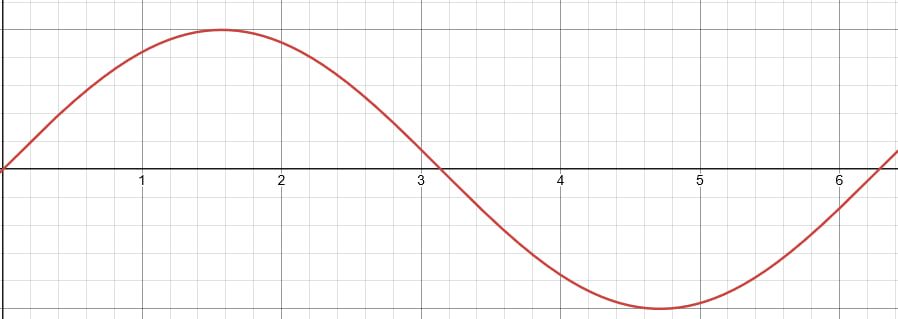
\includegraphics[height=100px]{2.2.jpg}

    \subsection{Убедитесь в линейной независимости фундаментальной системы решений данного ДУ, выпишите вронскиан.}
    \begin{equation*}
        W=[y_1, y_2] = 
        \begin{vmatrix}
            e^{-2x}(\cos x + \sin x) && e^{-2x}(\cos x - \sin x)\\
            -e^{-2x}(\cos x + 3\sin x) && e^{-2x}(\sin x -3\cos x)
        \end{vmatrix}
        =
    \end{equation*}
    \begin{equation*}
        =  e^{-2x}(\cos x + \sin x)(e^{-2x}(\cos x + \sin x - \sin x - \cos x)) - e^{-2x}(\cos x - \sin x)(e^{-2x}(\cos x + \sin x - \sin x + \cos x)) = 
    \end{equation*}
    \begin{equation*}
         = 2e^{-4x} \cos x(\cos x - \sin x)
    \end{equation*}
    Существует интервал $[\frac{\pi}{12}, \frac{5 \pi}{12}]$ на котором вронскиан не нулевой $\Rightarrow$ система линейно независима
    
    \subsection{Составьте линейное неоднородное дифференциальное уравнение (ЛНДУ) с правой частью $f (t) =
    t^2e^{2t}$. Выясните физический смысл функции $f (t)$.}
    Данная $f(t)$ отражает колебания - затухающее\\
    $y''(t) + 4y'(t) + 5y(t) = t^2e^{2t}$ - ЛНДУ

    \subsection{Решите ЛНДУ методом вариации произвольных постоянных.}
    $y''(t) + 4y'(t) + 5y(t) = t^2e^{2t}$ - ЛНДУ\\
    $y_{O.O} = e^{-2t}(D_1 \cos t + D_2 \sin t$\\
    $f(t) = t^2 e^{2t} = e^{2t} M_2 (t)$, тогда\\
    $y_0 = e^{2t} (A t^2 + B t + C$\\
    $y_0' = 2e^{2t}(A t^2 + B t + C) + e^{2t}(2A t + B) = 
    e^2t(2A t^2 + (2A + 2B)t + (2C + B))$\\
    $y_0'' = e^2t(2A t^2 + (2A + 2B)t + (2C + B)) + e^{2t}(4A t + (2A + 2B)) = e^{2t}(4A t^2 + (8A + 4B)t + (2A + 4B + 4C))$\\
    \begin{equation*}
        \begin{cases}
            4A + 2A + A = 1\\
            8A + 4B + 2A + 2B + B = 0\\
            2A + 4B + 4C + 2C + B + C = 0
        \end{cases}
        \begin{cases}
            A = \frac{1}{7}\\
            10A + 7B = 0\\
            2A + 5B + 7C = 0
        \end{cases}
        \begin{cases}
            A = \frac{1}{7}\\
            B = - \frac{10}{7 \cdot 7} \\
            7C = -2A -5B
        \end{cases}
        \begin{cases}
            A = \frac{1}{7}\\
            B = - \frac{10}{49} \\
            7C = -2A -5B
        \end{cases}
        \begin{cases}
            A = \frac{1}{7}\\
            B = - \frac{10}{49} \\
            C = \frac{36}{49}
        \end{cases}
    \end{equation*}
    $y=e^{-2t}(D_1 \cos t + D_2 \sin t) + e^{2t}(\frac{1}{7}t^2 - \frac{10}{49}t + \frac{36}{49})$
    
    
    
    

% task 3
\newpage
    \section{Дана система линейных дифференциальных уравнений 1-го порядка:
    \begin{equation*}
        \begin{cases}
            y' = z + \cos x, \\
            z' = 2y + z + 5 \sin x
        \end{cases}
    \end{equation*}
    Найдите методом исключения общее решение этой системы.
    }
    $z_x' = \frac{dz}{dx}(y'- \cos x) = y_{xx}'' + \sin x$

    \begin{equation*}
        z = y' - \cos x\\
        z' = 2y + z + 5 \sin x
    \end{equation*}
    $y'' + \sin x = 2y + (y' - \cos x) + 5 \sin x$\\
    $y'' - y' -2y = 4 \sin x - \cos x$\\
    Общее однородное: $\lambda^2 - \lambda -2 = 0$\\
    $\lambda_1 = 2, \lambda = -1$\\
    $y_{O.O} = C_1 e^{2x} + C_2 e^{-x}$\\
    $y_{0} = A \sin x + B \cos x$\\
    $y_{0}' = A \cos x - B \sin x$\\
    $y_{0}'' = - A \sin x - B \cos x$\\
    $(-A \sin x - B \cos x) - (A \cos x - B \sin x) - 2 (A \sin x + B \cos x) = 4 \sin x - \cos x$\\
    \begin{equation*}
        \begin{cases}
            -3A + B = 4\\
            A + 3B = 1
        \end{cases}
    \end{equation*}
    \begin{equation*}
        \begin{cases}
            A = -1.1\\
            B = 0.7
        \end{cases}
    \end{equation*}
    $y_{0} = - 1.1 \sin x + 0.7 \cos x$\\
    $y_{O.H} = C_1 e^{2x} + C_2 e^{-x} - 1.1 \sin x + 0.7 \cos x$\\
    $z = y' - \cos x$\\
    $y' = 2C_1 e^{2x} - C_2 e^{-x} - 1.1 \cos x - 0.7 \sin x$\\
    $z = 2C_1 e^{2x} - C_2 e^{-x} - 2.1 \cos x - 0.7 \sin x$
    \begin{equation*}
        \text{Ответ:}
        \begin{cases}
            y = 2C_1 e^{2x} - C_2 e^{-x} - 1.1 \cos x - 0.7 \sin x\\
            z = 2C_1 e^{2x} - C_2 e^{-x} - 2.1 \cos x - 0.7 \sin x
        \end{cases}
    \end{equation*}


% task 4
\newpage
    \section{Примените операционный метод для решения следующих задач Коши:}

    \subsection{
    \begin{equation*}
    \begin{cases}
        x' = -2y -3e^{-2t}, \; x(0) = -1,\\
        y' = 2x - 4y - 2e^{-2t}, \; y(0) = -1        
    \end{cases}
    \end{equation*}
    }
    $x(t)\rightarrow X(p)$ \\
    $x'(t)\rightarrow pX(p) - x(p) = X(p)p +1$ \\
    $y(t) \rightarrow Y(p)$ \\
    $y'(t) \rightarrow pY(p) +1 $\\
    $e{^{(-2t)}} \rightarrow \frac{1}{p+2}$\\
    
    \begin{equation*}
    \begin{cases}
        pX + 1 = -2Y - \frac{3}{p+2}\\
        pY + 1 = 2X - 4Y - \frac{2}{p+2}      
    \end{cases}
    \end{equation*}
    \begin{equation*}
    \begin{cases}
        pX = -2Y - \frac{p+5}{p+2}\\
        pY = 2X -4Y - \frac{p+4}{p+2}     
    \end{cases}
    \end{equation*}
    \begin{equation*}
    \begin{cases}
        2Y = -pX -\frac{p+5}{p+2}\\
        (p+4)Y = 2X - \frac{p+4}{p+2}    
    \end{cases}
    \end{equation*}
    \begin{equation*}
    \begin{cases}
        Y = -\frac{p}{2}X - \frac{p+5}{2(p+2)} \\
        \frac{-p(p+4)}{2}X - \frac{(p+4)(p+5)}{2(p+2)} = 2X - \frac{p+4}{p+2}
    \end{cases}
    \end{equation*}
     \begin{equation*}
    \begin{cases}
        X\frac{(p+2)^2}{2} = \frac{(p+4)}{p+2} -\frac{(p+5)(p+4)}{2(p+2)}\\
        Y = -\frac{p}{2}x - \frac{p+5}{2(p+2)}
    \end{cases}
    \end{equation*}
    \begin{equation*}
    \begin{cases}
        X\frac{(p+2)^2}{2} = \frac{(p+4)(2-p-5)}{2(p+2)}\\
        Y = -\frac{p}{2}x - \frac{p+5}{2(p+2)}
    \end{cases}
    \end{equation*}
     \begin{equation*}
    \begin{cases}
        X = -\frac{(p+4)(p+3)}{(p+2)^3}\\
        Y = \frac{(p+4)(p+3)p}{(p+2)^3 2} - \frac{p+5}{2(p+2)}
    \end{cases}
    \end{equation*}
    \begin{equation*}
    \begin{cases}
        Y = -\frac{1}{p+2} - \frac{2}{(p+2)^2} - \frac{2}{(p+2)^3}\\
        X = -t^2 e^{-2t} - 3te^{-2t} - e^{-2t}
    \end{cases}
    \end{equation*}
    \begin{equation*}
        \begin{cases}
            x(t) = -t^2 e^{-2t} - 3t e^{-2t} - e^{-2t}\\
            y(t) = -t^2 e^{-2t} - 2t e^{-2t} - e^{-2t}
        \end{cases}
    \end{equation*}

    \subsection{
    \begin{equation*}
        x''+2x'+17x=
        \begin{cases}
            136,\; t \in [0; 2), \; x(0) = -2,\\
            0,\; t \notin [0; 2), \; x'(0) = 10
        \end{cases}
    \end{equation*}
    }
    $x \rightarrow X(p)$ \\
    $x' \rightarrow pX(p) - A$ \\
    $x'' \rightarrow p^2 X(p) - Ap -B$ \\
    \begin{equation*}
        p^2X-Ap-B+pX-A+17x =
        \begin{cases}
            136,\; t \in [0; 2)\\
            0,\; t \notin [0; 2)
        \end{cases}
    \end{equation*}
    $X(p^2+p+17) - Ap - A - B = C$ \\
    $X(p^2 + p +17) = A(p+1) + B+C$\\
    \begin{equation*}
        C =
        \begin{cases}
            136,\; t \in [0; 2)\\
            0,\; t \notin [0; 2)
        \end{cases}
    \end{equation*}
    $X = \frac{A(p+1) +B+C}{p^2+p+17}$ \\
    $X = \frac{Ap}{p^2 + p +17} + (A+B+C) \frac{1}{p^2+p+17}$ \\
    $x(t) = A(e^{\frac{-t}{2}} \cos(\frac{\sqrt{67}}{2}t) - \frac{1}{\sqrt{67}} e^{\frac{-1}{2}t}\sin{\frac{\sqrt{67}}{2}t}) + (A+B+C)(\frac{2}{\sqrt{67}}e^{\frac{-1}{2}t}\sin{\frac{\sqrt{67}}{2}t})$, где\\
    \begin{equation*}
    \begin{cases}
        B = 0, A = -2, C = 136 \text{ при } t \in [0;2)\\
        B = 10, A = 0, C = 0 \text{ при }  t \notin [0;2)
    \end{cases}
    \end{equation*}

% evaluation paper
\newpage
\[
\renewcommand{\arraystretch}{2}
\begin{tabular}{| c | c |}
 \hline
    \hugeУчастник & \hugeВклад в \% \\
 \hline
    \hugeКаренин Константин & \huge25 \\
 \hline
    \hugeГонин Сергей & \huge25 \\
 \hline
    \hugeТемиров Тимур & \huge25 \\
 \hline
    \hugeМалышева Алиса & \huge25 \\
 \hline
\end{tabular}
\]
\end{document}